\subsection{4-1 ResetPrefix}

\subsubsection*{Questions}

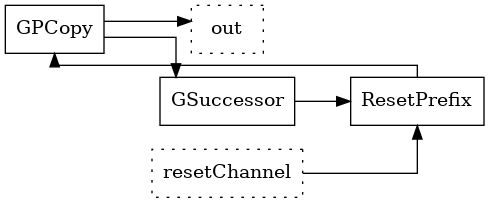
\includegraphics[width=\textwidth]{graphs/chapter4/4-1-1.png}

\paragraph{What happens if line {25} of ResetPrefix Listing 4-1 is commented out?}

If line 25 \mintinline{groovy}{inChannel.read()} is commented out then, after a reset, the output stream alternates between the two streams of numbers.

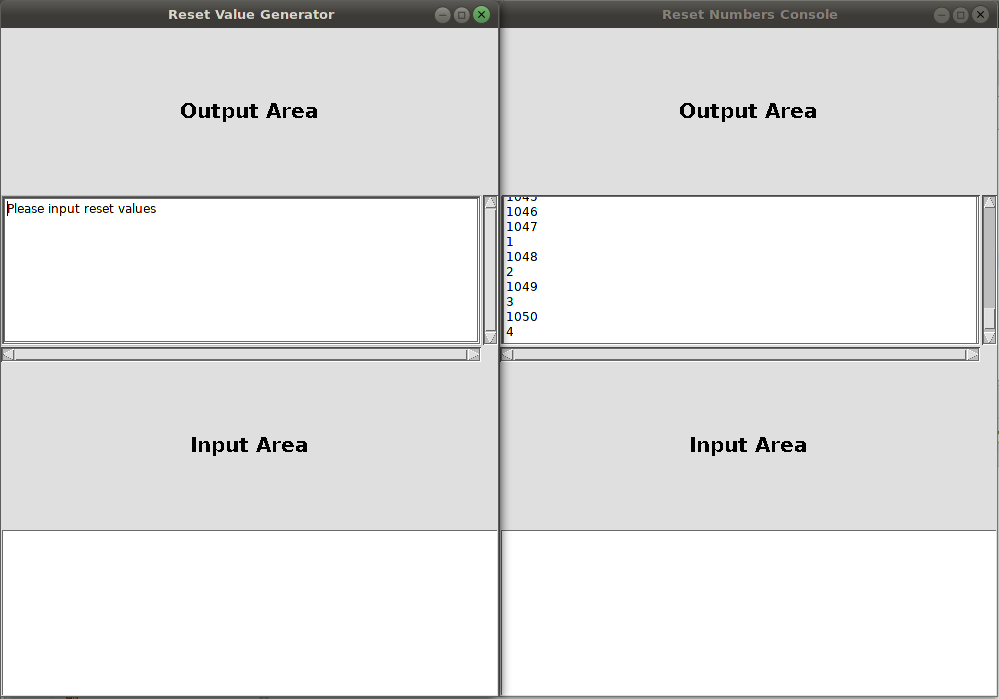
\includegraphics[width=\textwidth]{img/screenshots/4-1-1.png}

\paragraph{Why?}

\inputgroovy[label=ResetPrefix.groovy,firstline=21,lastline=31,numberblanklines=true]{../ChapterExamples/src/c04/ResetPrefix.groovy}

As can be seen in the while loop of ResetPrefix, if line 25 is commented out, the number is never removed from inChannel.  In the next iteration line 29 runs, reading the original value and writing it to the output value, this causes ResetPrefix to alternate between the two values as the original value is never discarded.